\chapter{User Interface}

\section{User Interface Draft 1}
	\label{uiDrafts} 

	\begin{figure}[H]
		\centering
		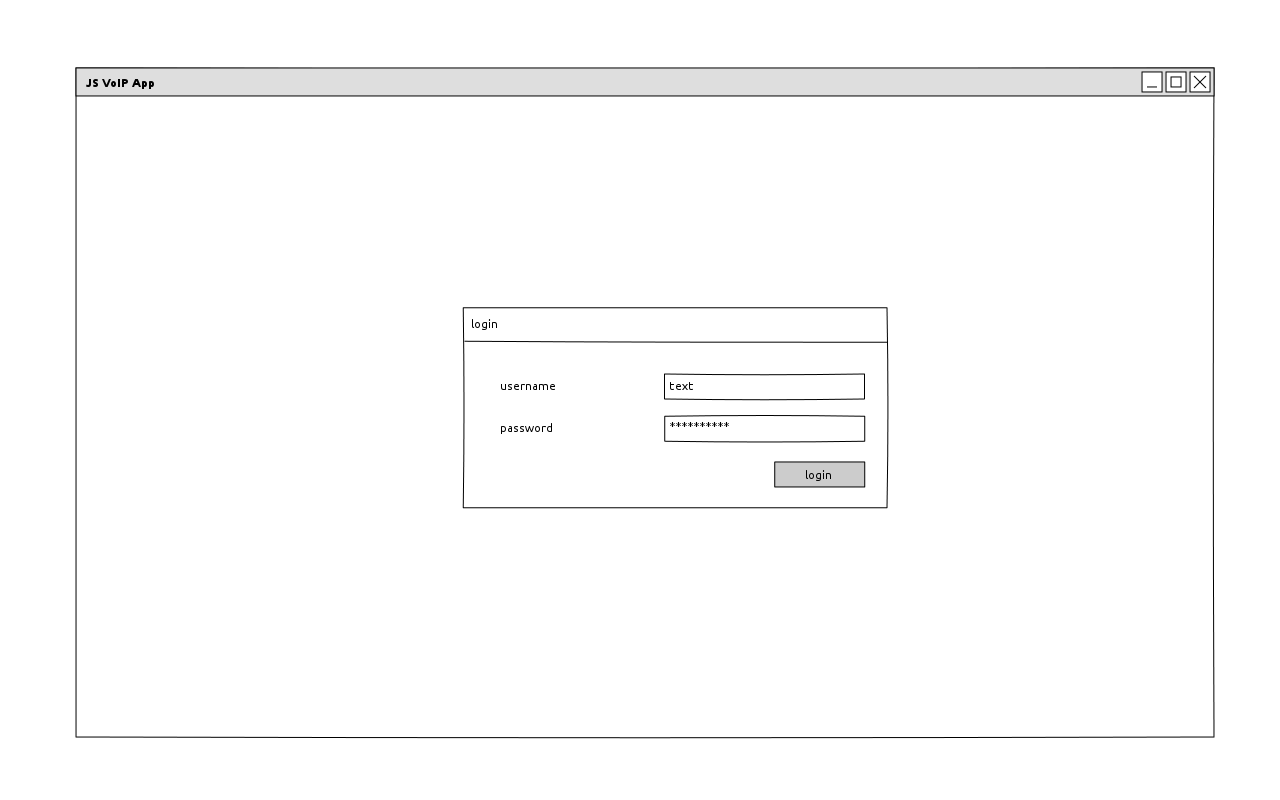
\includegraphics[height=0.3\textheight]{../ui/img/uiDraft1/login_page.png}
		\caption{Über den Login Screen loggen sich Benutzer ein.}
		\label{login screen}
	\end{figure}
	\begin{figure}[H]
		\centering
		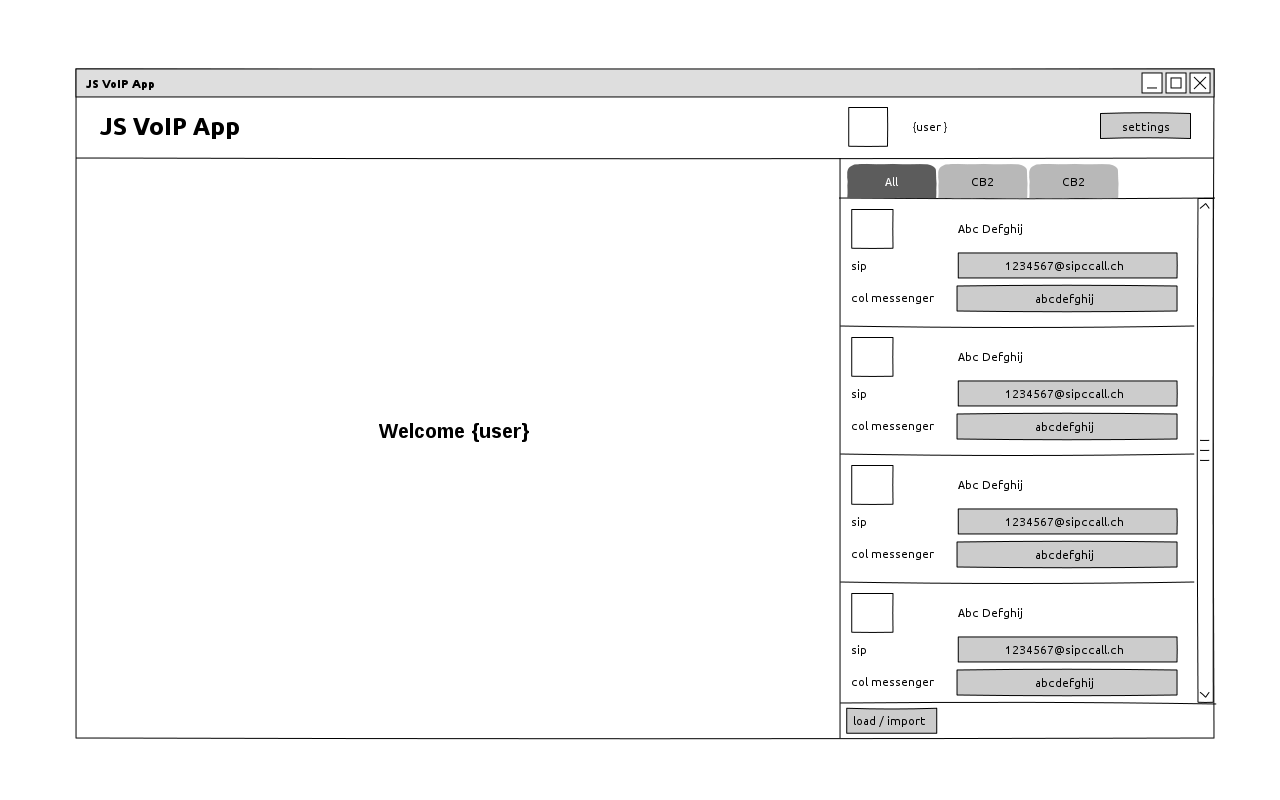
\includegraphics[height=0.3\textheight]{../ui/img/uiDraft1/main_view.png}
		\caption{In der Hauptansicht hat der Benutzer Zugriff auf das Adressbuch.}
		\label{main screen}
	\end{figure}
	\begin{figure}[H]
		\centering
		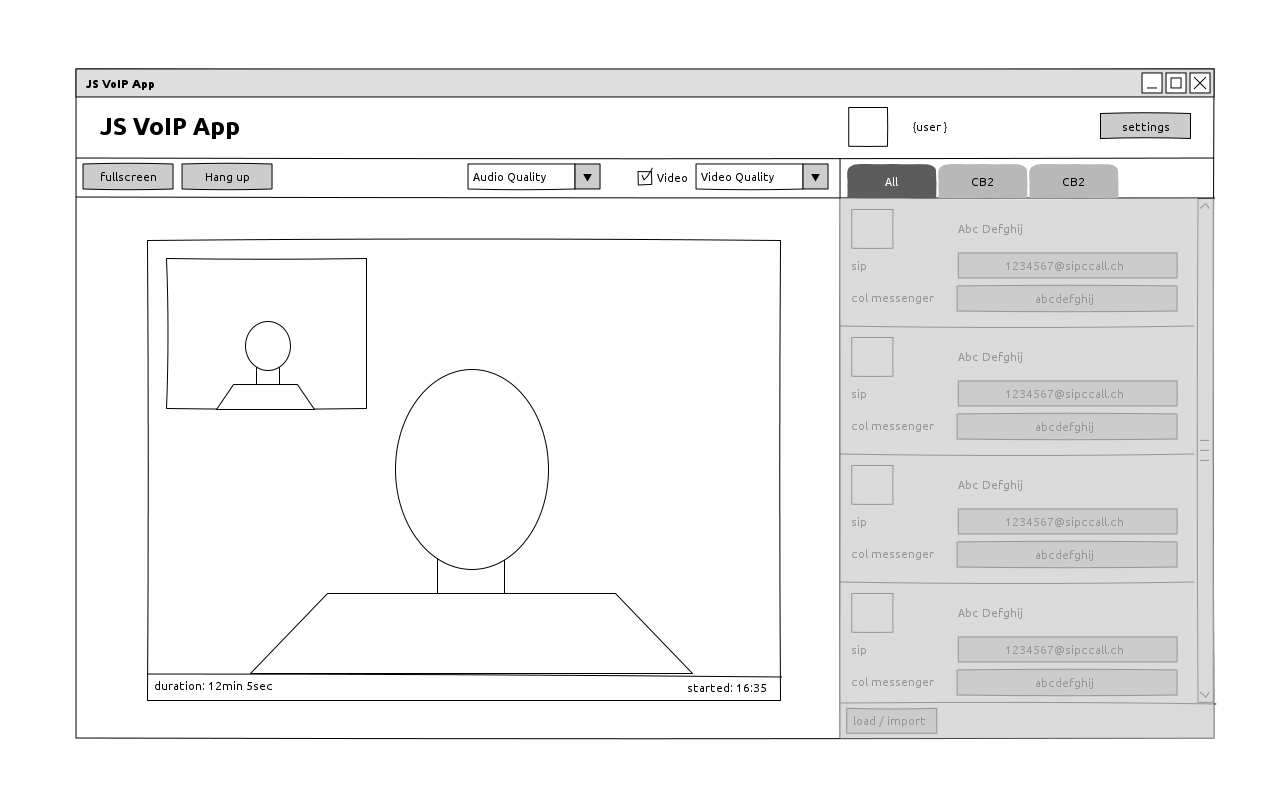
\includegraphics[height=0.4\textheight]{../ui/img/uiDraft1/call_view.png}
		\caption{Ruft der Benutzer einen Kontakt an, so wird das Video in der Hauptansicht eingeblendet und die Kontakte werden inaktiv.}
		\label{call screen}
	\end{figure}
	\begin{figure}[H]
		\centering
		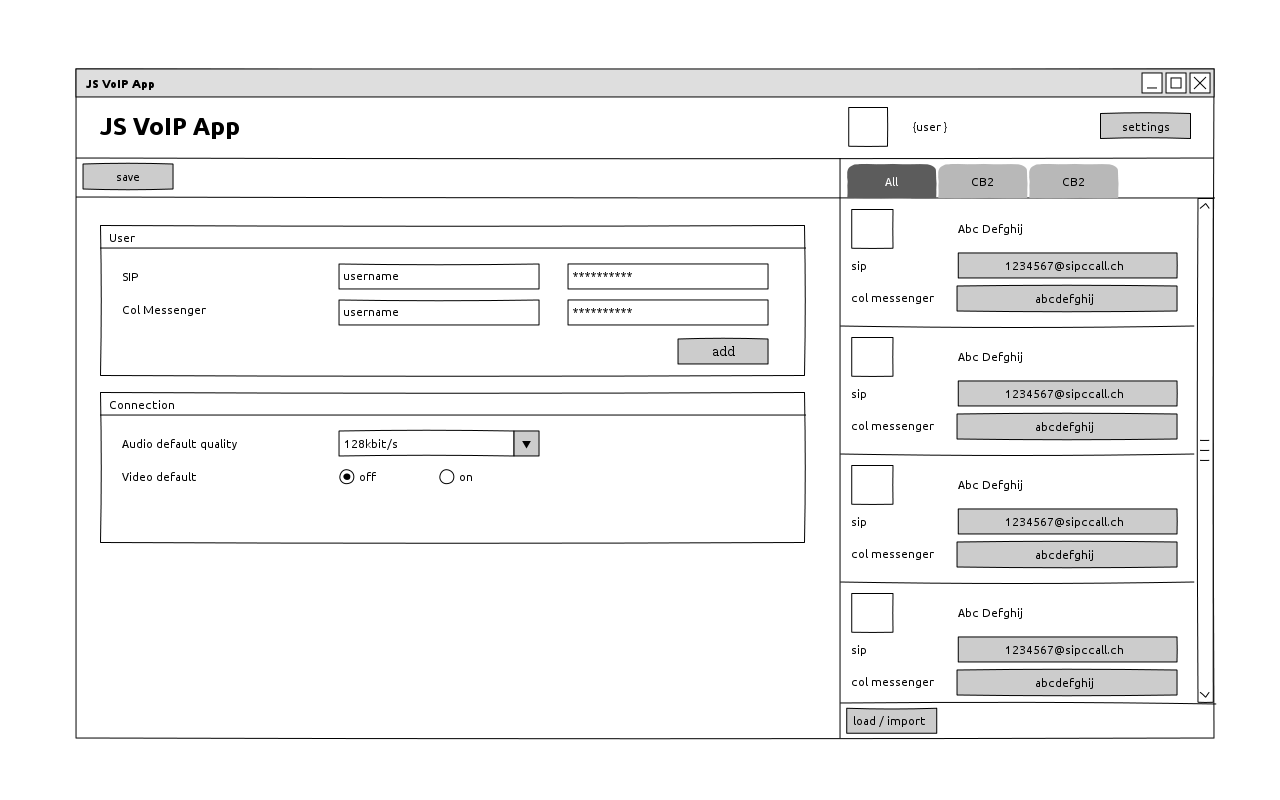
\includegraphics[height=0.4\textheight]{../ui/img/uiDraft1/settings_view.png}
		\caption{Über die Settings kann der Bentzer Einstellungen verändern.}
		\label{settings screen}
	\end{figure}
	
	
\section{User Interface Draft 2}
	Das UI2 folgt dem Prinzip ``Mobile First"'.
	\begin{figure}[H]
		\centering
		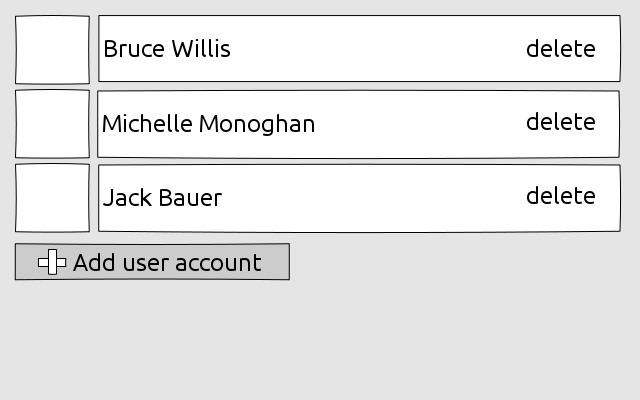
\includegraphics[height=0.35\textheight]{../ui/img/uiDraft2/UserView-selectUser.png}
		\caption{Benutzer Verwaltung und Login Screen. Durch klick auf einen Benutzer kann sich der Benutzer mit dessen Konto anmelden.}
		\label{login screen}
	\end{figure}
	\begin{figure}[H]
		\centering
		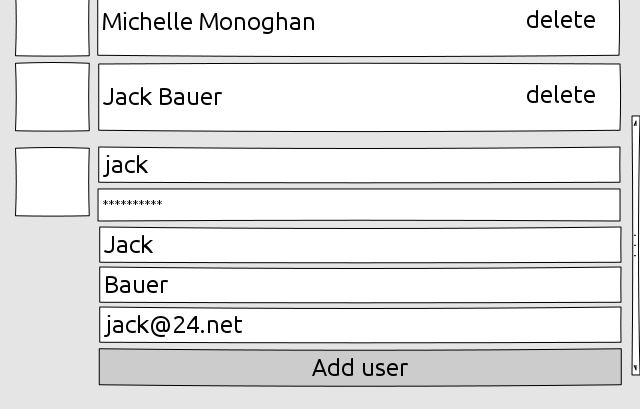
\includegraphics[height=0.35\textheight]{../ui/img/uiDraft2/UserView-addUser.png}
		\caption{Die Benutzerverwaltung erlaubt es dem benutzer auch gleich einen neuen Bentzer zu erfassen.}
		\label{user management screen}
	\end{figure}
		\begin{figure}[H]
		\centering
		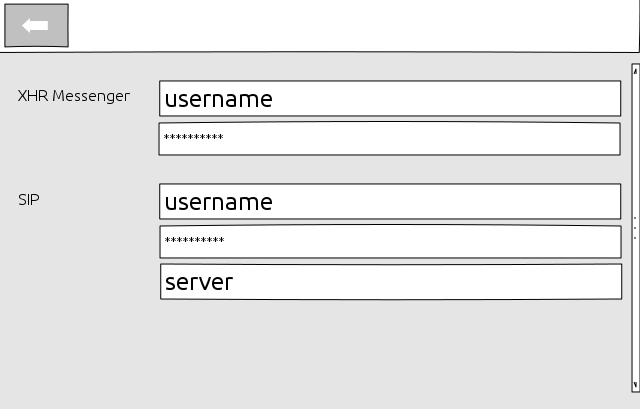
\includegraphics[height=0.4\textheight]{../ui/img/uiDraft2/UserView-addChannel.png}
		\caption{Die Bentzerverwaltung ermöglicht dem Benutzer das verwalten der verfügbaren Channel Accounts.}
		\label{user management screen}
	\end{figure}
	\begin{figure}[H]
		\centering
		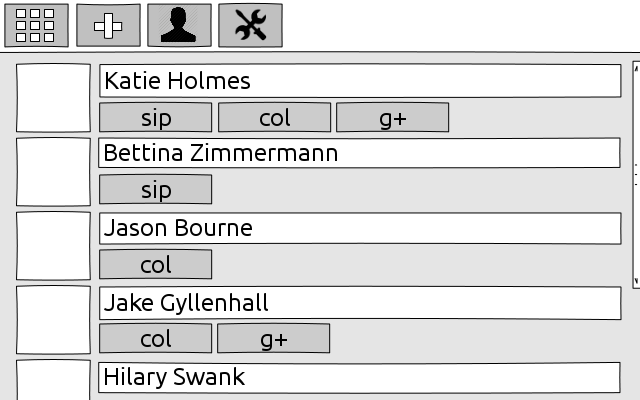
\includegraphics[height=0.4\textheight]{../ui/img/uiDraft2/ContactbookView.png}
		\caption{Adressbuch: Von hier aus ruft der Benutzer seine Kontakte an. Die verschiedenen Adressbücher sind über das Listensymbol erreichbar.}
		\label{contactbook screen}
	\end{figure}
	\begin{figure}[H]
		\centering
		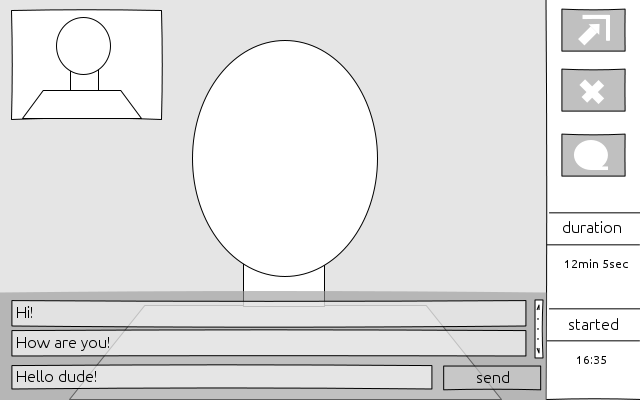
\includegraphics[height=0.4\textheight]{../ui/img/uiDraft2/PhoneViewWithMessenger.png}
		\caption{Phone View: Nebst dem Video sieht der Benutzer elementare Informationen über den Anruf.}
		\label{settings screen}
	\end{figure}
	\begin{figure}[H]
		\centering
		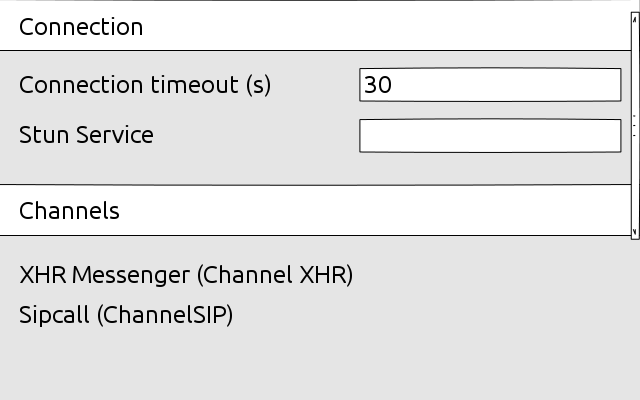
\includegraphics[height=0.4\textheight]{../ui/img/uiDraft2/SettingsView.png}
		\caption{In den Settings kann der Benutzer Konfiguration und Channels einsehen.}
		\label{settings screen}
	\end{figure}
	
\section{Finales User Interface}
	\begin{figure}[H]
		\centering
		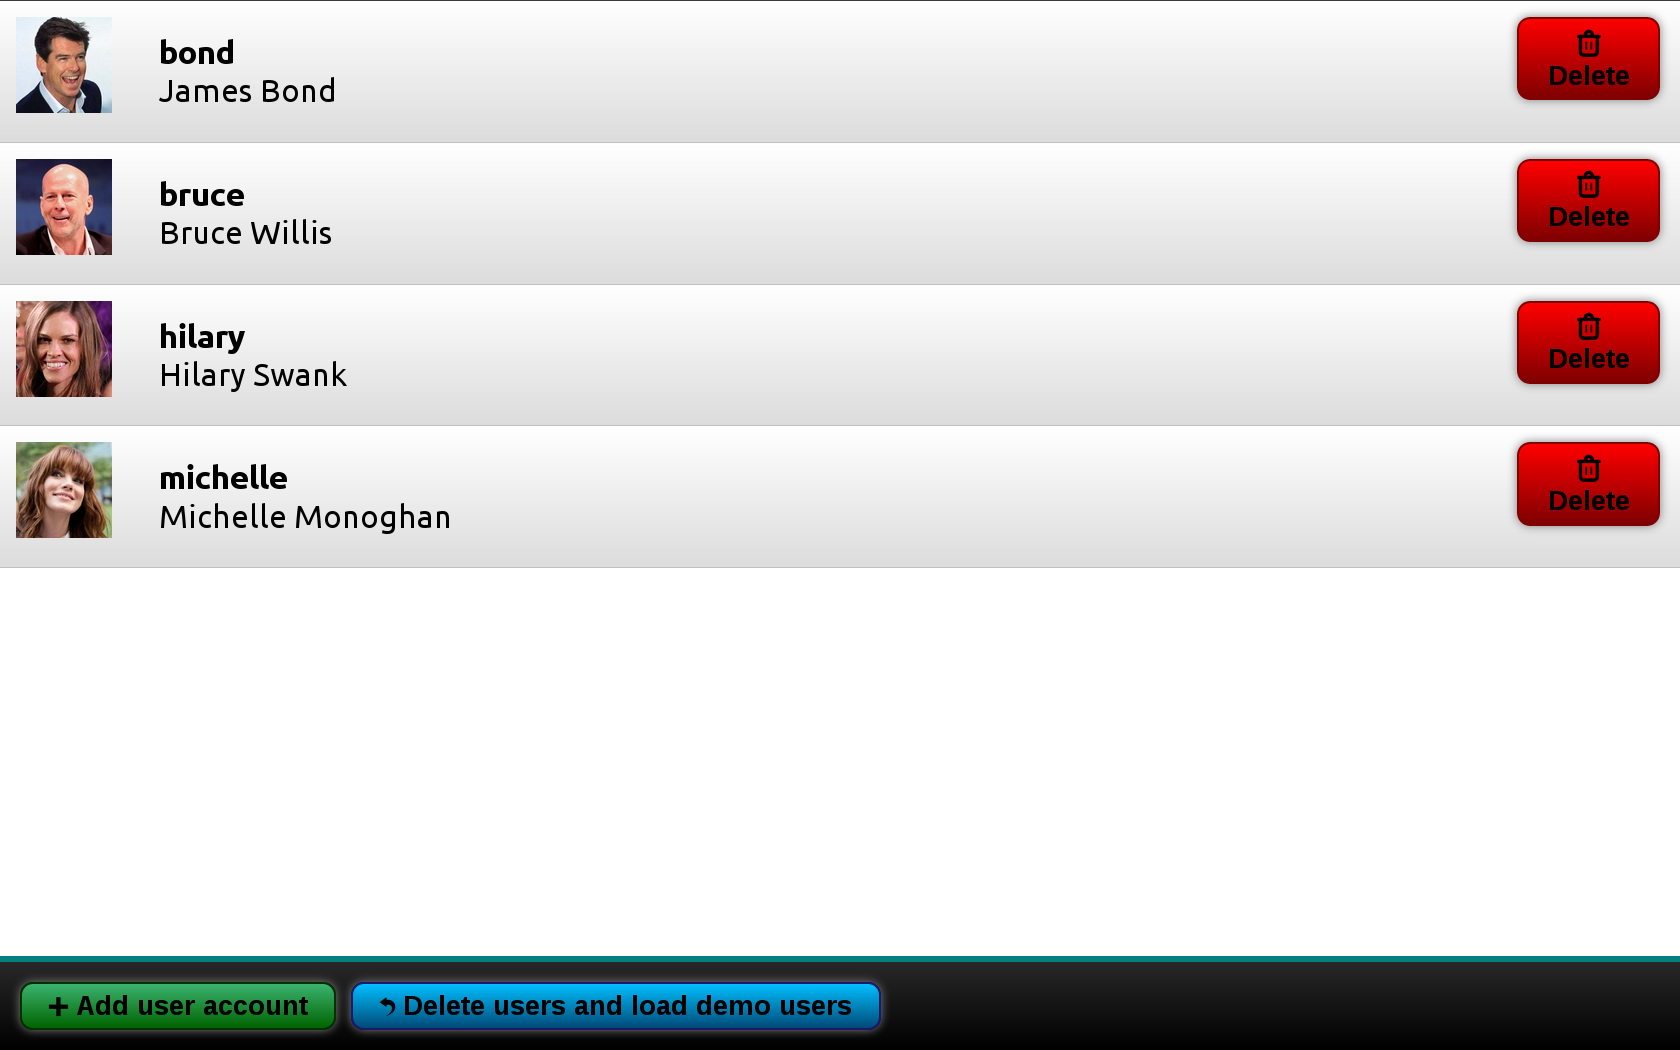
\includegraphics[height=0.35\textheight]{../ui/img/finalUi/accountView.png}
		\caption{Benutzer Verwaltung und Login Screen. Durch klick auf einen Benutzer kann sich der Benutzer mit dessen Konto anmelden.}
		\label{login screen}
	\end{figure}
	\begin{figure}[H]
		\centering
		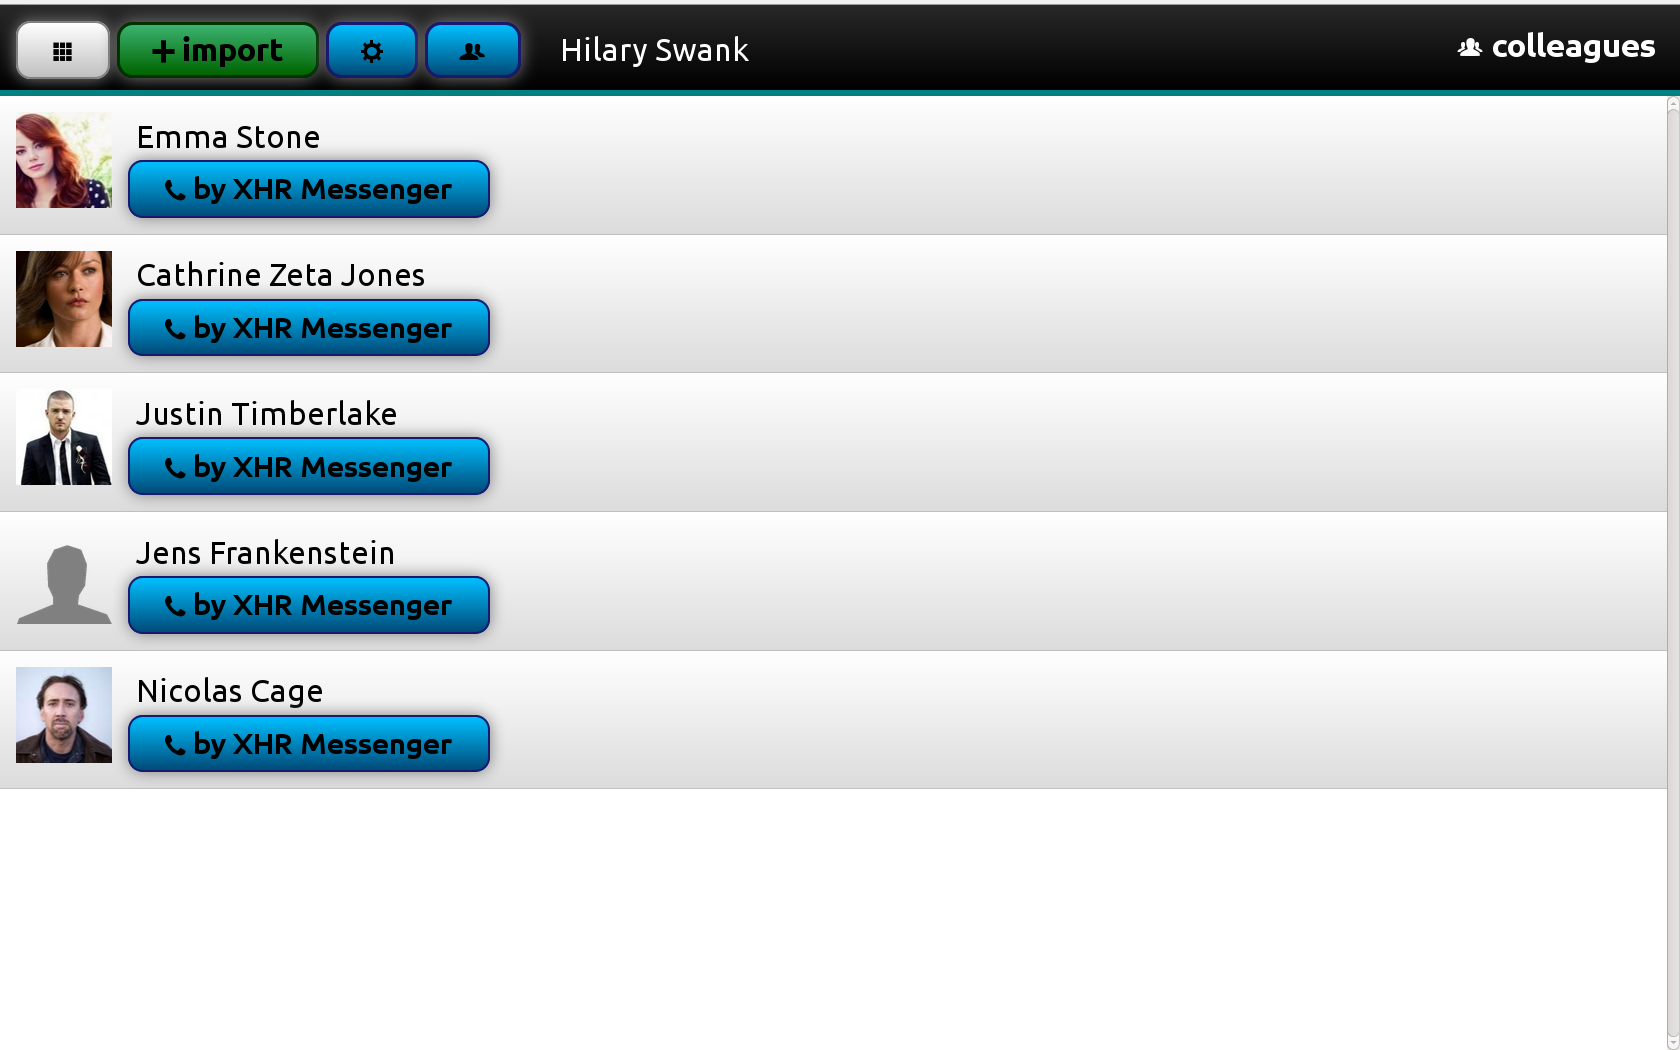
\includegraphics[height=0.35\textheight]{../ui/img/finalUi/contactView1.png}
		\caption{Adressbuch: Von hier aus ruft der Benutzer seine Kontakte an. Die verschiedenen Adressbücher sind über das Listensymbol erreichbar.}
		\label{contactbook screen}
	\end{figure}
	\begin{figure}[H]
		\centering
		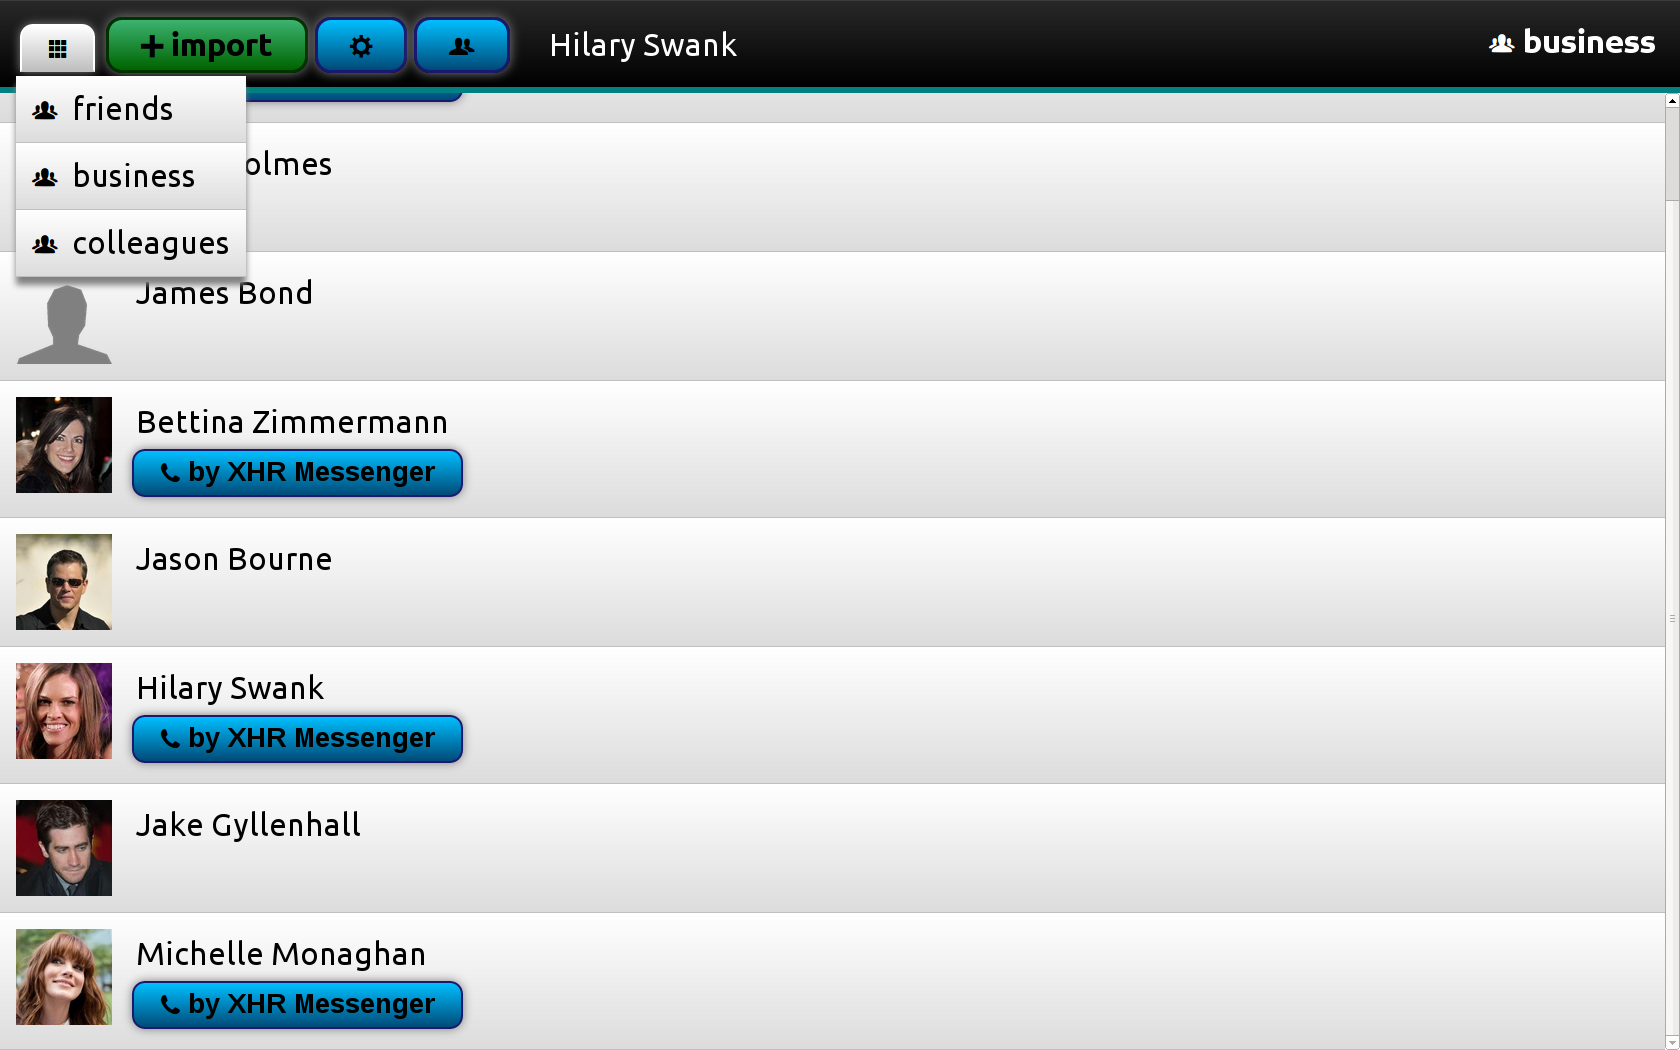
\includegraphics[height=0.4\textheight]{../ui/img/finalUi/contactView2.png}
		\caption{Auswahl des anzuzeigenden Adressbuches.}
		\label{contactbook change}
	\end{figure}
	\begin{figure}[H]
		\centering
		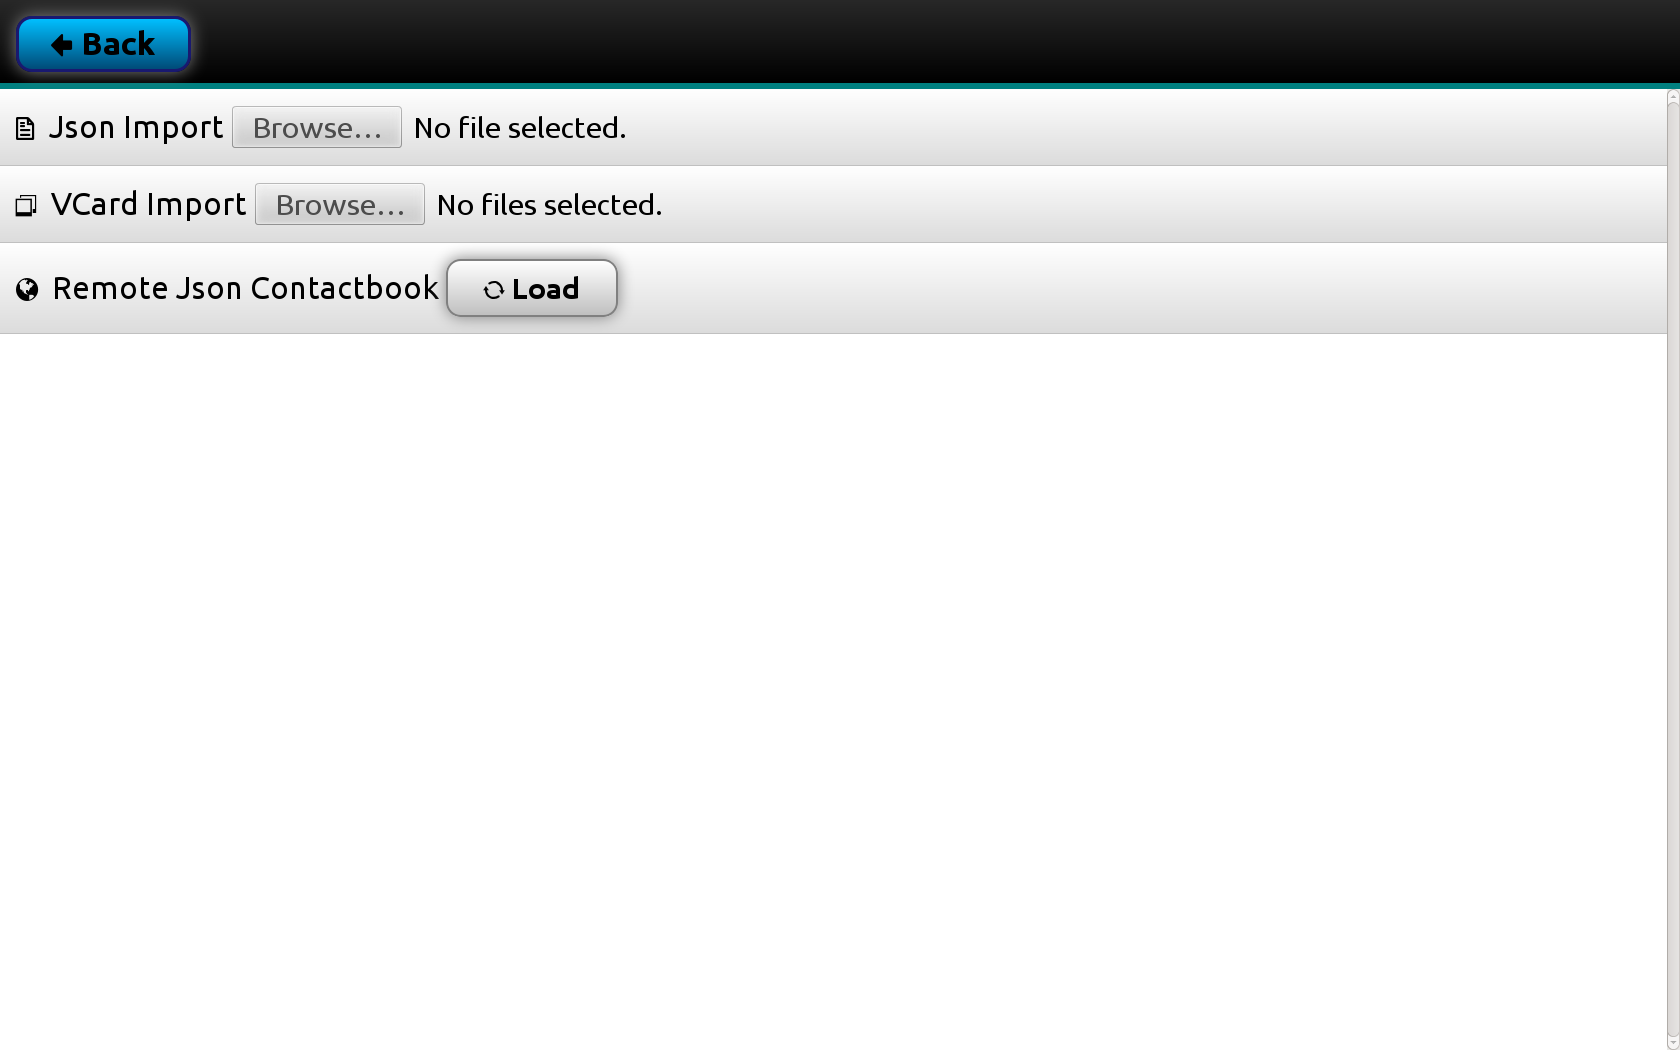
\includegraphics[height=0.4\textheight]{../ui/img/finalUi/importView.png}
		\caption{Adressbuch Import}
		\label{contactbook import screen}
	\end{figure}
	\begin{figure}[H]
		\centering
		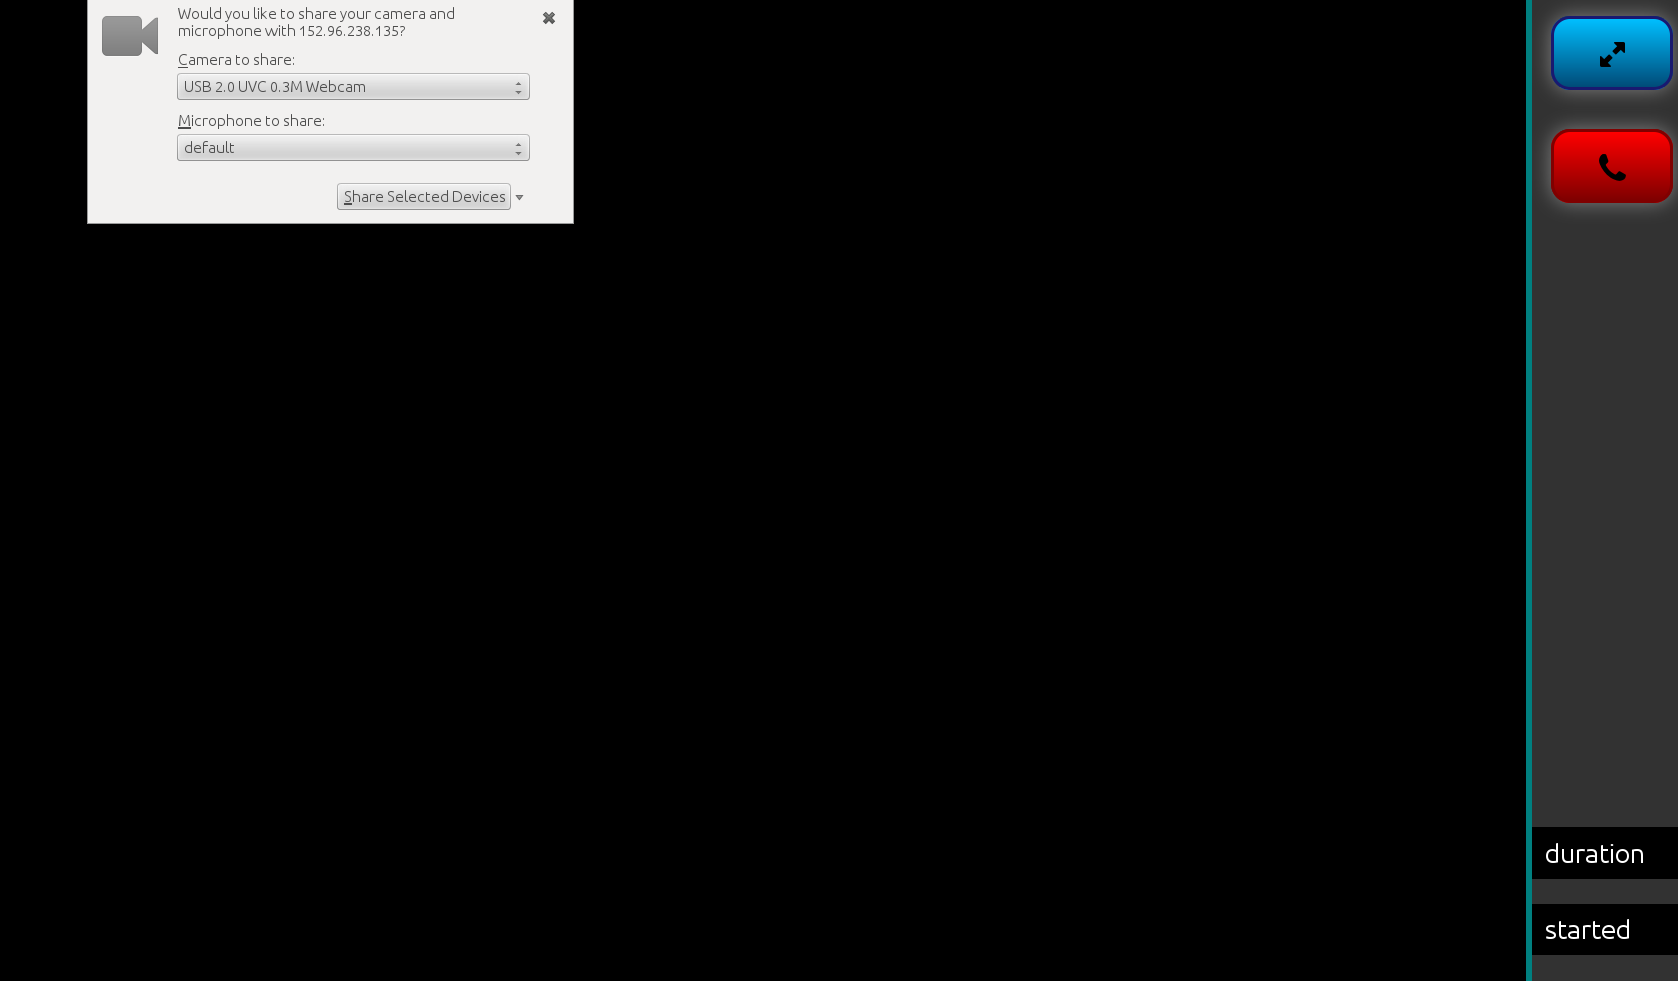
\includegraphics[height=0.4\textheight]{../ui/img/finalUi/cameraAccess.png}
		\caption{Anrufen: Kamerazugriff}
		\label{phone screen camera access}
	\end{figure}
	\begin{figure}[H]
		\centering
		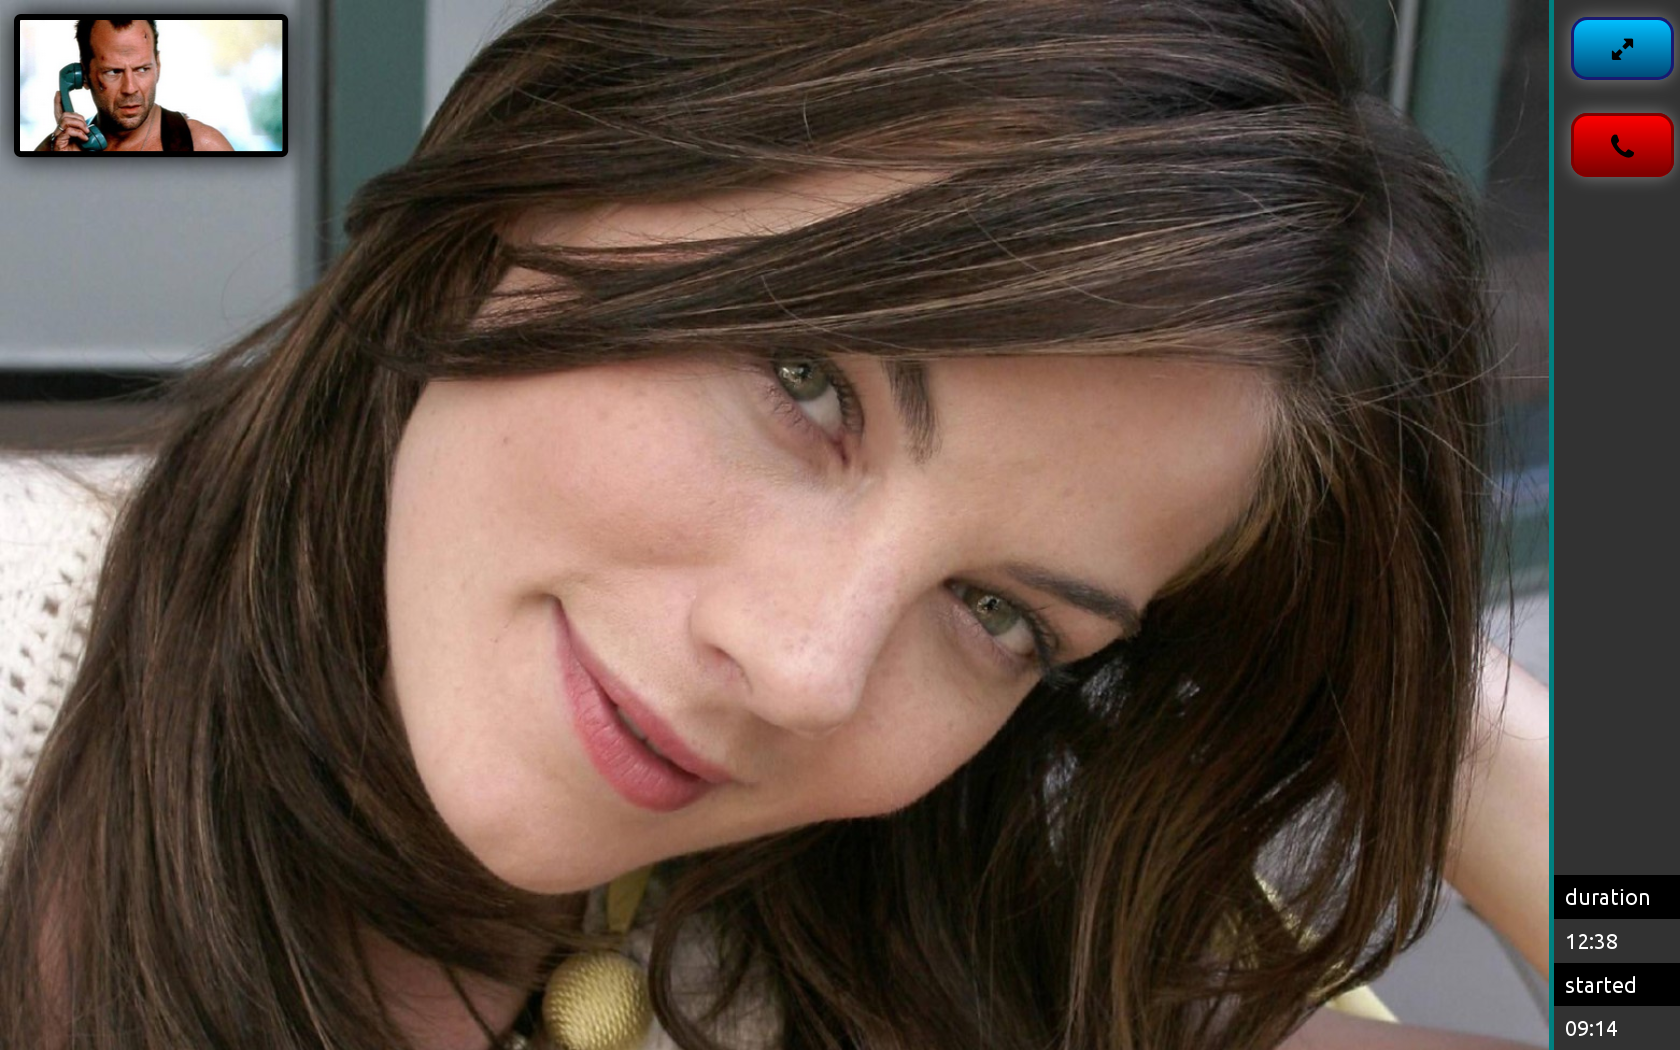
\includegraphics[height=0.4\textheight]{../ui/img/finalUi/phoneView.png}
		\caption{Anrufen}
		\label{phone screen}
	\end{figure}
	\begin{figure}[H]
		\centering
		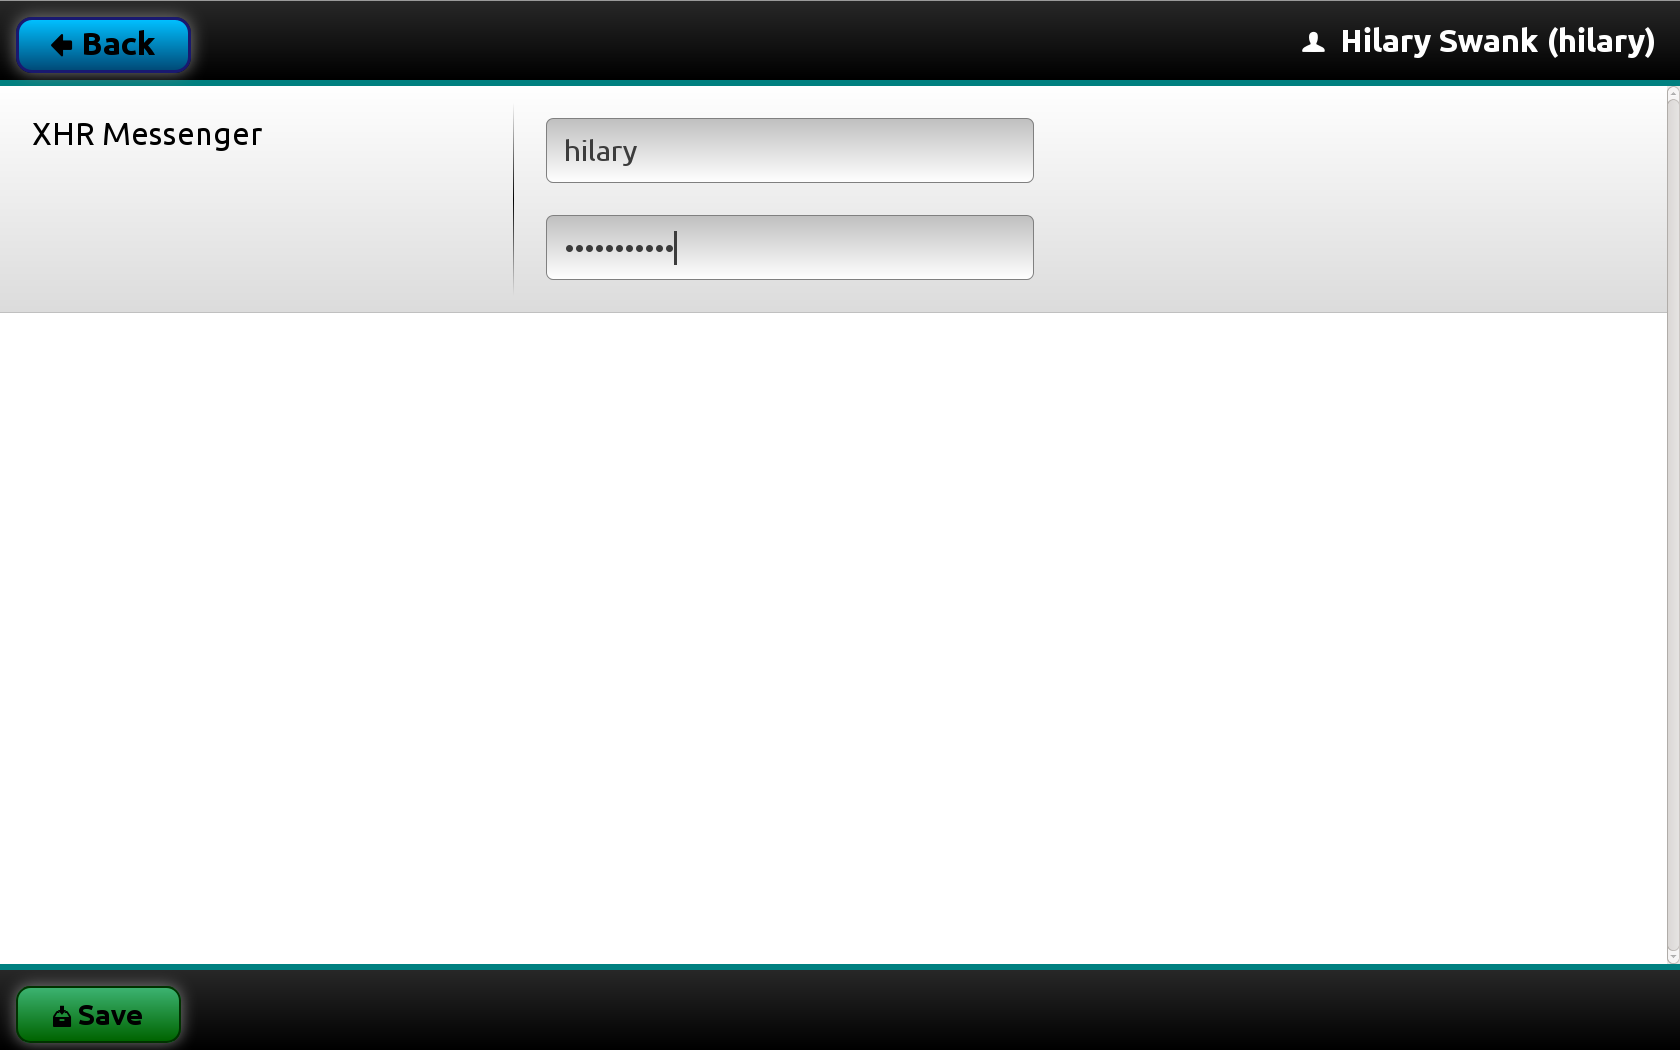
\includegraphics[height=0.4\textheight]{../ui/img/finalUi/accountEditView.png}
		\caption{Account Setting: Verwaltung der Zugänge der aktiven Channels}
		\label{account edit screen}
	\end{figure}